\documentclass[12pt,twoside,a4paper]{scrartcl}

\usepackage{prakstyling}
\usepackage[paper=a4paper,left=20mm,right=20mm,top=20mm,bottom=20mm]{geometry}
\usepackage{wrapfig}
\usepackage{amsmath}
%Für Literaturverzeichnis

\usepackage{biblatex}
\addbibresource{Bibliography.bib}



%%%%%%%%%%%%%%%%%%%%%%%%%%%%%%% Autoreninfo %%%%%%%%%%%%%%%%%%%%%%%%%%%%%%%%%%%%%%%%%%%%%%%%%%
\author{Philipp Rosendahl Mat.-Nr: 378029\thanks{philipp.rosendahl@rwth-aachen.de}
		\and Lennart Wilde, Mat.-Nr: 381588\thanks{lennart.wilde@rwth-aachen.de}}

\pSetShortAuthor{378029 \& 381588}
%%%%%%%%%%%%%%%%%%%%%%%%%%%%%%%%%%%%%%%%%%%%%%%%%%%%%%%%%%%%%%%%%%%%%%%%%%%%%%%%%%%%%%%%%%%%%

%%%%%%%%%%%%%%%%%%%%%%%%%%%%%%%%%%%%%%%% TITEL %%%%%%%%%%%%%%%%%%%%%%%%%%%%%%%%%%%%%%%%%%%%%%
\pSetTitlePrefix{Versuch}
\pSetTitleNumber[PET]
\pSetLongSubject{Physikalisches Fortgeschrittenenpraktikum - Gruppe 59} \pSetShortSubject{Gruppe 59}
%%%%%%%%%%%%%%%%%%%%%%%%%%%%%%%%%%%%%%%%%%%%%%%%%%%%%%%%%%%%%%%%%%%%%%%%%%%%%%%%%%%%%%%%%%%%%

\setlength{\parindent}{0pt}
\pagenumbering{roman}

\raggedbottom

\renewcommand{\tablename}{Tab.}
\renewcommand{\figurename}{Fig.}
\setlength{\abovecaptionskip}{1ex}
\setlength{\belowcaptionskip}{1ex}
\setlength{\floatsep}{1ex}
\setlength{\textfloatsep}{1ex}

\begin{document}

\maketitle
\newpage

\tableofcontents
\newpage

\pagenumbering{arabic}

\section{Einleitung}

	Die PET ist ein wichtiges Bildgebendes Verfahren in der modernen Medizin um auch kleine Tumore im menschlichen Körper ausfindig zu machen. Daher ist die Entwicklung leistungsfähiger Detektoren ein wichtiger Aspekt moderner Forschung. \\

	Das zugrunde liegende Prinzip basiert auf der besonders hohen Biologischen Aktivität von Tumorgewebe. Wir einem Patienten nun ein mit einem Radioaktiven Isotop markierter Zucker (sog. Tracer) verabreicht, sammelt sich dieser in dem Tumor an. Wenn dieser nun zerfällt emittiert er Positronen die sich mit den Elektronen im umliegenden Gewebe auslöchen und zwei Gamma Photonen in entgegengestezte Richtung aussenden. Diese sollen durch die Detektoren aufgefangen und ausgewertet werden um Informationen über Flugzeit und Energie der Strahlung zu erhalten. Für die Konstruktion dieser Detektoren gibt es mehrere Ansätze, allerdings wurde in diesem Experiment ein Silicon-Photomultiplier (SiPM) zusammen mit einem LYSO Szintillator verwendet.\\

	Ein auftreffendes Gamma-Photon regt den Szintillierenden Kristall nun an optische Photonen auszusenden, die auf den SiPM treffen. Dort werden sie in ein elektrisches Signal umgewandelt, welches durch einen ASIC ausgelesen und verarbeitet werden kann, um aus der Anzahl der Photonen die Energie des detektierten Photons sowie die Flugzeit udn Position zu rekonstruieren. In einem medizinischen PET-Scanner kann mit diesen Informationen nun die Lage der Tumoren im Patienten errechnet werden. In diesem Versuch ist allerdings eher die Vermessung des verwendeten Detektors im Fokus, weswegen nur zwei sich gegenüberstehende Detektoren verwendet werden.

	\newpage

\section{Versuchsaufbau}

	Der Aufbau besteht aus verschiedenen Teilen:
	\begin{itemize}
		\item Dunkelbox mit
		\begin{itemize}
			\item 2 $\gamma$-Detektoren
			\item Backbone
			\item Aluminiumgstell mit Schrittmotoren für Probenhalter
			\item Probenhalter für Radioaktive Probe
			\item
		\end{itemize}
		\item Netzteile für Detektoren und Backbone
		\item Data Aquisition and Processing Server (DAPS)
		\item Kühlung
		\item Steuerungsrechner mit Benutzerinterfaces
	\end{itemize}

	\begin{figure}[H]
		\centering
		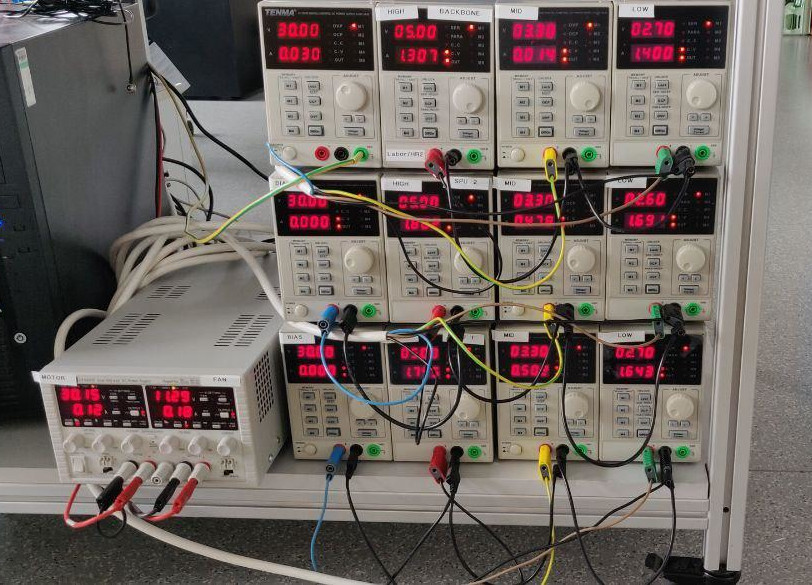
\includegraphics[width = 0.7\textwidth]{Pictures/Netzteile.jpg}
		\label{Aufbau::Netzteile}
		\caption{Netzteile mit verschiedenen Spannungen}

	\end{figure}

	\begin{figure}[H]
		\begin{minipage}{0.69\textwidth}

					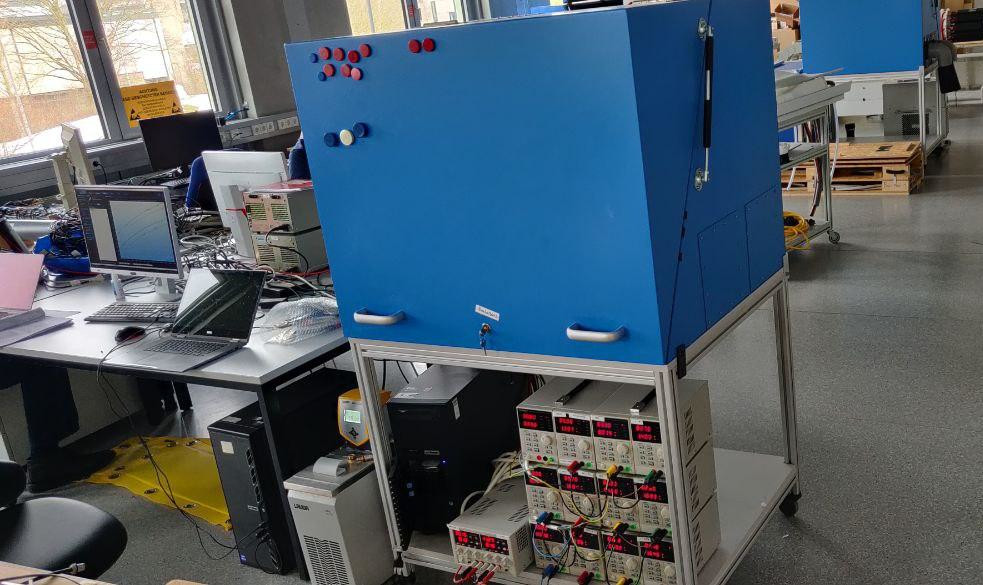
\includegraphics[width = 0.8\textwidth]{Pictures/Kammer.jpg}
					\label{Aufbau::Kammer}
					\caption{Geöffnete Dunkelkammer}

		\end{minipage}
		\begin{minipage}{0.3\textwidth}

					\includegraphics[width = 0.8\textwidth]{Pictures/Kühlung.jpg}
					\label{Aufbau::Kühlung}
					\caption{Wasserkühlung}
		\end{minipage}
	\end{figure}


	Um den Aufbau einzuschalten, muss zuerst die Kühlung gestartet werden. Danach werden die LOW, MID und HIGH Spannungen des Backbone in dieser Reihenfolge eingeschaltet. Daraufhin bootet dieser, wobei der vollständige Start durch einen Sprung in der Stromaufnahme der HIGH-Versorgungsspannung festgestellt werden kann. Nachdem der Backbone gestartet ist, können die 2 Detektoren (SPUs) eingeschaltet werden, indem wie schon bei dem Backbone zuerst die Versorgungsspannungen in der Oben angegebenen Reihenfolge sowie die BIAS-Spannung eingeschaltet werden. Auch hier ist die Betriebsbereitschaft durch einen Sprung in der Stromaufnahme auf ungefär 1.6 A erkennbar. Nun kann der Steuerungsrechner mit dem Aufbau verbunden werden. Dazu startet man die \glqq Hyperion\grqq \ Software und führt dort das zu dem Versuch gehörenden Startskript aus. Daraufhin wird eine Verbindung hergestellt, die Detektoren initialisiert und mit dem Backbone synchronisiert. Aufgrund von sporadisch auftretenden Verbindungsproblemen zwischen Backbone und den SPUs kann dieser Schritt fehlschlagen, worauf dann die Spannungen un der umgekehrten Reihenfolge abgeschaltet und der Aufbau neu gestartet werden muss.
	Ist erfolgreich eine Verbindung zwischen allen Komponenten hergestellt, sollte spätenstens nun die Dunkelkammer geschlossen werden, da im nächsten Schritt die Bias-Spannungen an die SiPMs angeschlossen werden. Wären diese nun nicht im dunklen würden sie konstant ausgelöst, was Messungen unmöglich macht und sie außerdem beschädigen kann. Ist die Kammer also geschlossen, kann mit dem Skript \glqq Continue\_Start \grqq der Aufbau in einen Messbereiten Zustand versetzt werden.

	\section{Kalibration des Probenhalters}

		\subsection{Ziel}
			Da die Steuerungssoftware mit eigenen Einheiten (nachfolgend \glqq Pulse\grqq genannt) arbeitet, muss zuerst ermittelt werden wie sich diese zu dem tatsächlich verfahrernen Strecken des Probenhalters verhalten.

		\subsection{Aufbau und Durchführung}
			Am unteren Ende des Schlittens, auf dem sich der Probenhalter befindet, ist eine Ablesenadel für einen Metermaßstab angebracht. Der entsprechende Maßstab ist unter dieser aud dem Aluminiumprofil des Aufbaus angebracht. Zum Start der Messung wird der Motor mittels der Kontrollsoftware in seine Startposition gebracht, bei der er 0 Pulse verfahren ist. Dann lässt man diesen 5000 Pulse vorfahren und liest die Aktuelle Position des Schlitten auf dem Maßstab ab. Dies wird so lange wiederholt, bis der Schlitten am Endstop Schalter auf der anderen Seite angekommen ist.

		\subsection{Auswertung}

			Es wurden bei der Messung folgende Daten aufgenommen:

				\begin{table}[H]
    \centering
    \caption{Rohdaten Kalibration}

    \begin{tabular}{| c | c |}
      Pulse & Strecke in $\si{\per \centi \metre}$ \\
                              \hline
                              0 &	35.35 \\
                           5000 &	33.3 \\
                           10000 &	31.1 \\
                           15000 &	29.0 \\
                           20000 &	26.95 \\
                          25000 &	24.75 \\
                          30000 &	22.7 \\
                           35000 &	20.53 \\
                           \hline
    \end{tabular}
\end{table}



			Es ist sinnvoll anzunehmen dass die verfahrene Strecke und die ausgegebenen Pulse in einem linearen Zusammenhang stehen, daher wird die Modellfunktion
			\begin{align*}
					s = m \cdot x + b
			\end{align*}
			angenommen.
			Mitilfe eines Python Skriptes wird nun die Funktion an die aufgenommenen Messdaten gefittet:

			\begin{figure}[H]
				\centering
				%\includegraphics[width = 0.7\textwidth]{Plots/Calib_Fit.eps}
				\caption{Gradenanpassung an gemessene Daten}
			\end{figure}

				Damit folgt ein Umrechnungsfaktor von $m = (??? \pm ???) \frac{\si{\centi \metre}}{\text{Puls}}$ bei einem Offset von $b = (??? \pm ???) \si{\centi \metre}$.


	\section{Dark Count Map}
	\label{DCM}

		\subsection{Aufbau und Durchführung}

			Aufgrund des thermischen Rauschens der Dioden, sowie Herstellungsprzessen und -ungenauigkeiten haben diese eine sog. \glqq Dunkelzählrate\grqq, d.h. eine Signalausgabe bei nicht vorhandener Stimulation. Um nun einzelne Dioden mit besonders hoher Rate zu erkennen und abzuschalten, wird vor der ersten Messung eine \glqq Dark Count Map\grqq der SiPMs ohne eine Probe erstellt. Mithilfe dieser kann man nun ermitteln welche SPADs abgeschaltet werden sollten, um eine Reduzierung der Dunkelzählrate ohne eine zu hohe Reduktion der anderen Genauigkeiten zu errreichen.\\
			Zur Durchführung der Messung wird der Aufbau wie oben beschrieben eingeschaltet und das Skript zum Aufnehmen der Messung gestartet. Dies dauert einige Minuten, und nach Abschluss werden die Daten auf dem DPAS gespeichert und müssen von dort auf den Rechner übertragen werden.

		\subsection{Auswertung}

			Die aus der Messung erhaltenen Daten lagen als eine Datei mit Tab seperierten Werten (TSV) vor (siehe Rochdatenverzeichnis). Um eine einfache Übersicht über die Sensoren zu erhalten wurde die Datei nun meit einem Python Skript eingelesen und die enhalten Zählraten in einer 2D-Grafik angezeigt:

			\begin{figure}[H]
				\begin{minipage}{0.49 \textwidth}
					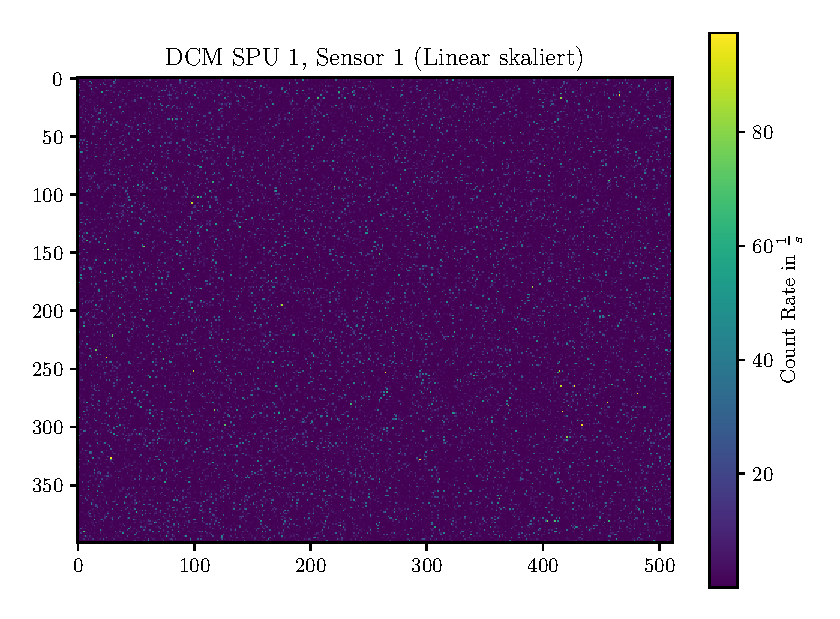
\includegraphics[width = \textwidth]{Plots/DCM/DCM_SPU1_Sensor1_lin.eps}
					\caption{Dark Count Map von SPU 1, Sensor 1}
				\end{minipage}
				\begin{minipage}{0.49 \textwidth}
					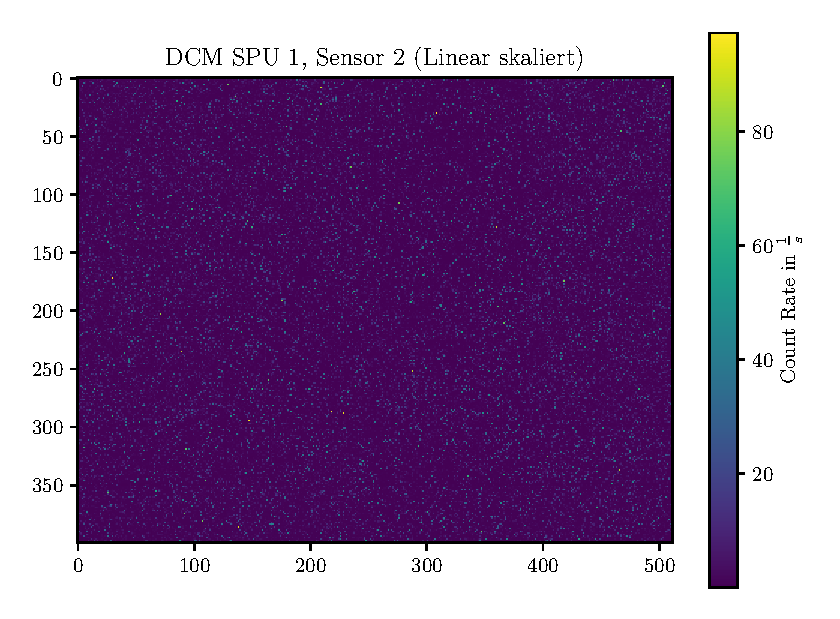
\includegraphics[width = \textwidth]{Plots/DCM/DCM_SPU1_Sensor2_lin.eps}
					\caption{Dark Count Map von SPU 1, Sensor 2}
				\end{minipage}
			\end{figure}

			\begin{figure}[H]
				\begin{minipage}{0.49 \textwidth}
					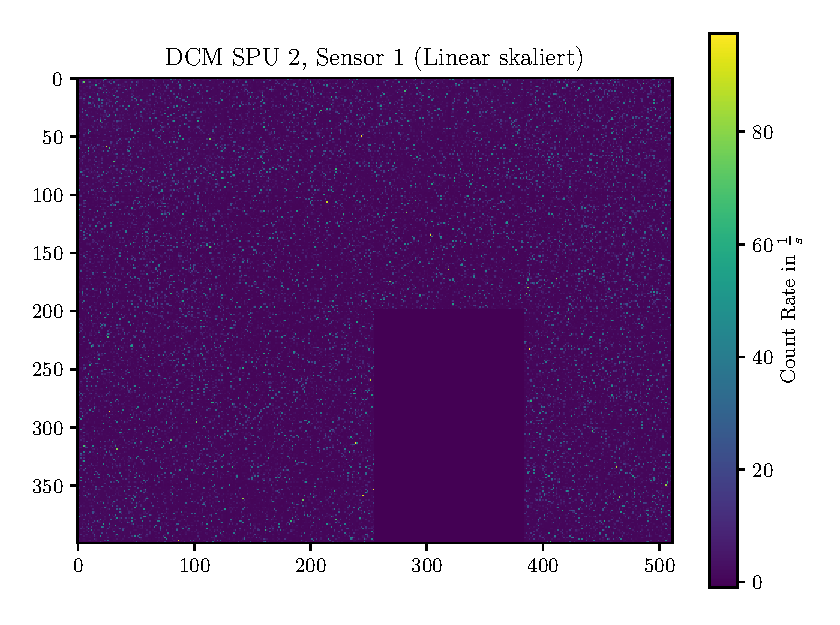
\includegraphics[width = \textwidth]{Plots/DCM/DCM_SPU2_Sensor1_lin.eps}
					\caption{Dark Count Map von SPU 2, Sensor 1}
				\end{minipage}
				\begin{minipage}{0.49 \textwidth}
					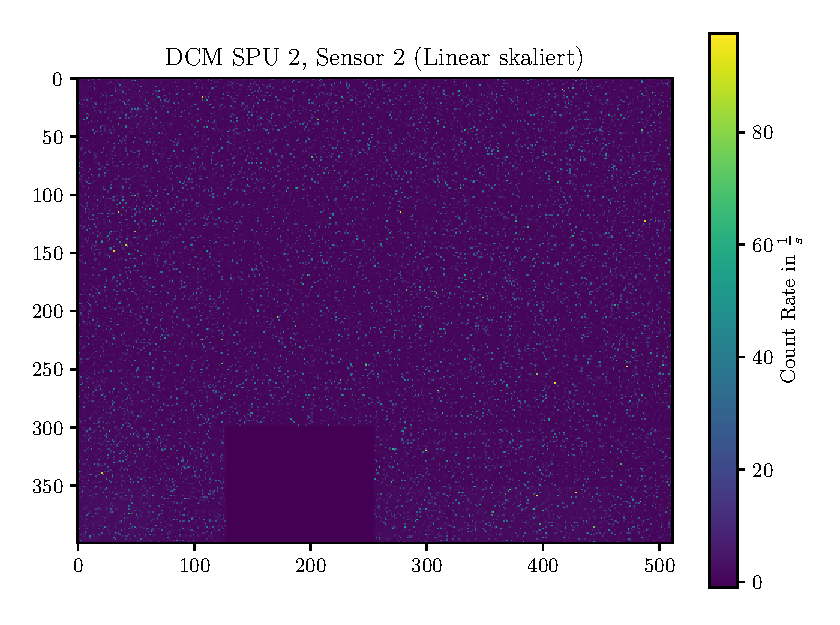
\includegraphics[width = \textwidth]{Plots/DCM/DCM_SPU2_Sensor2_lin.eps}
					\caption{Dark Count Map von SPU 2, Sensor 2}
				\end{minipage}
			\end{figure}
			Man kann erkennen dass die SPADs der Sensoren im allgemeinen geringe Dark Count Rates aufweisen, wobei einige wenige, den großteil der gesamten Rate ausmachen.
			In den Messdaten von SPU 2 ist auffällig, dass Cluster von SPADs ausgefallen sind, was auch in den Rohdaten der Messung so vorzufinden ist, sodass ein Auswertungsfehler unwahrscheinlich ist.
			Außerdem wird auf den Anhang \ref{Anhang} verwiesen in dem die Plots noch einmal größer und linear sowie logarithmisch skaliert zu finden sind.

			Außerdem wurde die Gesamtzählrate in Abhängigkeit von den abgeschalteten SPADs, wobei SPADs mit höherer Zählrate früher abgeschaltet wurden, ermittelt:

			\begin{figure}[H]
				\centering
				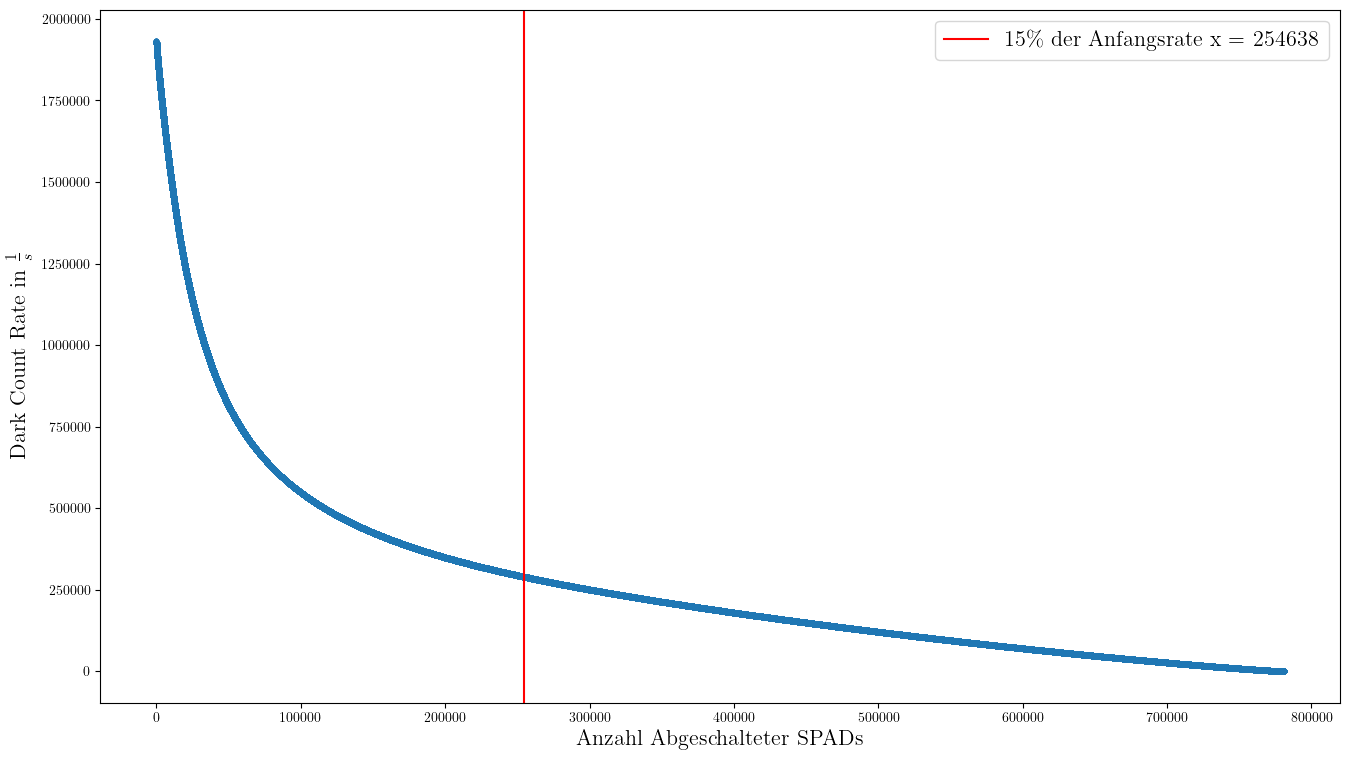
\includegraphics[width = 0.9 \textwidth]{Plots/DCM/DCR_vs_N.png}
				\caption{Dunkelzählrate der SPUs}
			\end{figure}

		\subsection{Fazit}

		Man sieht das N SPADs für einen Großteil des Rauschens sorgen der durch die Abschaltung dieser eliminiert werden kann. Für die weiteren Messungen ist sies leider nicht sonderlich relevant, da für die Sensoren vorkonfigurierte Prarameter verwendet wurden, in die wir leider keine Einsicht hatten.

	\section{Rauschmessung}

	\subsection{Ziel}

		Da sowohl das im Szintillator enthaltene Lutetium selbst radioaktiv ist, als auch die Umgebung eine natürliche Strahlenbelastung aufweist, ist es nötig vor der ersten Messung eine Rauschmessung vorzunehmen um die statistischen Messfehler des Detektors abschätzen zu können.

	\subsection{Aufbau und Durchführung}

		Der Aufbau wird wie schon im Abschnitt \ref{DCM} ohne das radioaktive Präparat hochgefahren, und es wird gewartet bis sich die Temperatur der SPUs stabilisiert hat.
		Dann wird mit dem Skript \glqq Start Scan\grqq die Messung gestartet und die Ansicht in der Hyperion-Software auf das Energie Histogramm gewechselt. Dort sind dann die Histogramme für einzeln auftreffende Photonen (Singles) und Koinzident auftreffende Photonen (Coincidences) sichtbar. Nach einigen Minuten kann die Messung mit \glqq Stop Scan\grqq beendet werden, und beide Histogramme werden gespeichert.

		\subsection{Auswertung}

		Die in der gespeicherten Datei enthaltenen Daten werden durch ein Python Porgramm aufbereitet und ausgewertet.
		Es folgen Plots für die Energie-Histogramme von Singles und Koinzidenten.

		\begin{figure}
				\begin{minipage}{0.49 \textwidth}
					%\includegraphics[width=\textwidth]{Plots/Energy_Hist_Singles.eps}
					\caption{Histogramm Singles}
				\end{minipage}
				\begin{minipage}{0.49 \textwidth}
						%\includegraphics[width=\textwidth]{Plots/Energy_Hist_Co.eps}
						\caption{Histogramm Koinzidenzen}
					\end{minipage}
		\end{figure}

		Man kann hier deutlich sehen dass kaum Koinzidenzen gemessen werden, was darauf schließen lässt dass die Photonen nicht aus einem Ereignis stammen.
		Außerdem kann mit diesen Messungen das Hintergrundrauschen der Singles gut eliminiert werden.

		\subsection{Fazit}

		\textbf{TODO}

	\section{Detektorsensitivität und Count Rate}

		\subsection{Aufbau und Durchführung}

			Das radioaktive Na-22 Präparat wird in den Probenhalter eingesetzt, und die minimalen Abstände der Probe zu dem beiden Sensoren vermessen. Nun wird die Dunkelbox geschlossen und der Aufbau wie schon in den beiden vorherigen Abschnitten eingeschaltet. Nachdem sich wieder eine stabile Temperatur an den Sensoren eingestellt hat, wird der Schlitten mit dem Probenhalter in die Mitte zwischen den beiden Detektoren verfahren und um diesen Punkt so mittels einer binären Suche so lange verfahren bis die Summe der Count-Rate der Detektoren maximal ist. Anschließend wurde das Messystem zurückgesetzt und die Count-Rate der Sensoren gespeichert.

		\subsection{Auswertung}

			Um die Detektorsensitivität zu bestimmen, kann man die theoretische Aktivität der Probe mit der tatsächlich gemessenen vergleichen.
			Dabei ist allerdings zu beachten dass durch die begrenzte Detektorfläche nur ein gewisser Anteil der tatsächlich abgestrahlten Positronen auch gemessen werden kann.
			Unter der Annahme dass die Positronen gleichmäßig unter allen Raumwinkeln abgestreut werden, muss nun als Korrekturfaktor der Anteil der Detektorfläche an der Fläche der Kugel mit dem Radius R, wobei dieser der Abstand zwischen Detektor und Probe ist, berechnet werden.

			\begin{align*}
				A_{\text{Detektor}} = \int_0^a \int_0^a 1 \dd{x} \dd{y} \\
				\frac{A_{\text{Detektor}}}{A_{\text{Kugel}}} = \\
			\end{align*}

		\subsection{Fazit}

	\section{Energiemessung}


	\section{Anhang}
		\label{Anhang}

		\subsection{Dark Count Maps}

		\begin{figure}[H]
			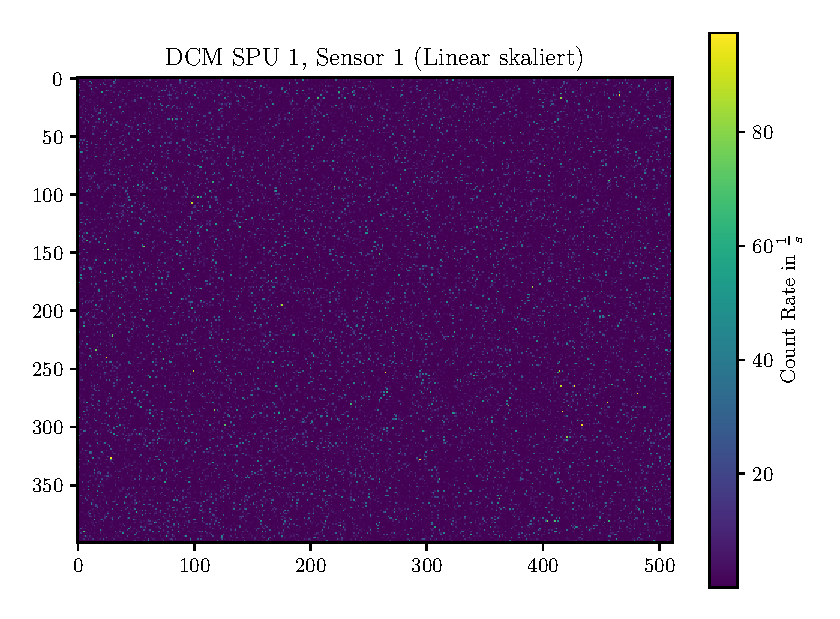
\includegraphics[width = \textwidth]{Plots/DCM/DCM_SPU1_Sensor1_lin.eps}
			\caption{DCM SPU 1, Sensor 1, Linear}
		\end{figure}

		\begin{figure}[H]
			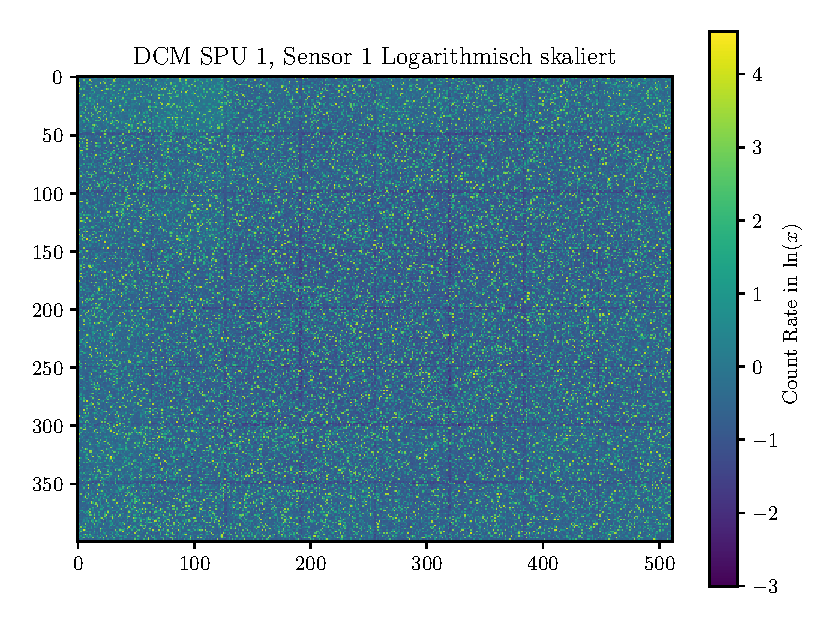
\includegraphics[width = \textwidth]{Plots/DCM/DCM_SPU1_Sensor1_log.eps}
			\caption{DCM SPU 1, Sensor 1, Logarithmisch}
		\end{figure}

		\begin{figure}[H]
			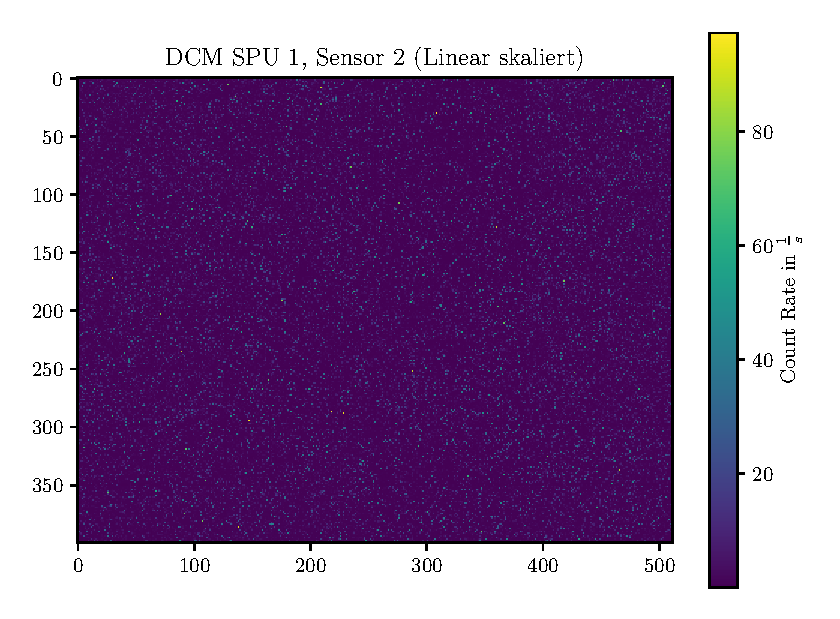
\includegraphics[width = \textwidth]{Plots/DCM/DCM_SPU1_Sensor2_lin.eps}
			\caption{DCM SPU 1, Sensor 2, Linear}
		\end{figure}

		\begin{figure}[H]
			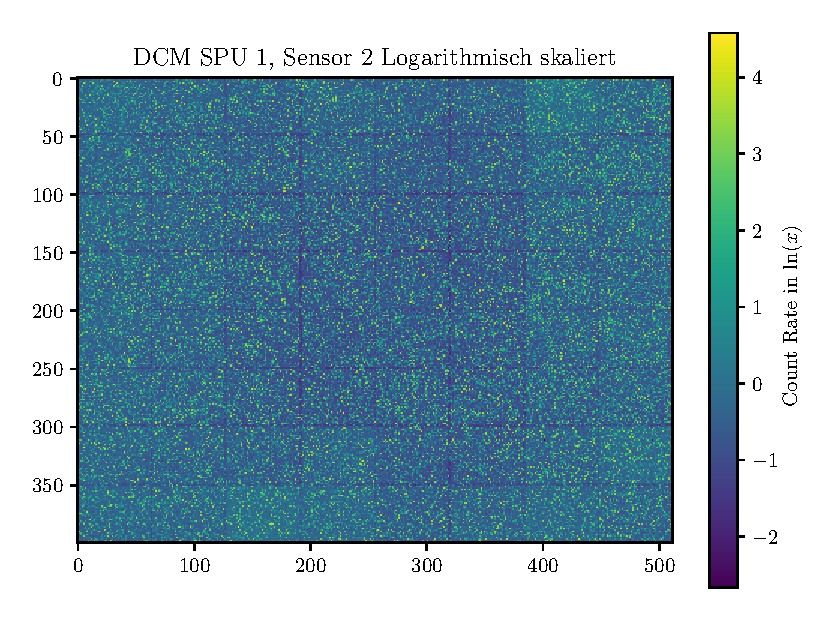
\includegraphics[width = \textwidth]{Plots/DCM/DCM_SPU1_Sensor2_log.eps}
			\caption{DCM SPU 1, Sensor 2, Logarithmisch}
		\end{figure}

		\begin{figure}[H]
			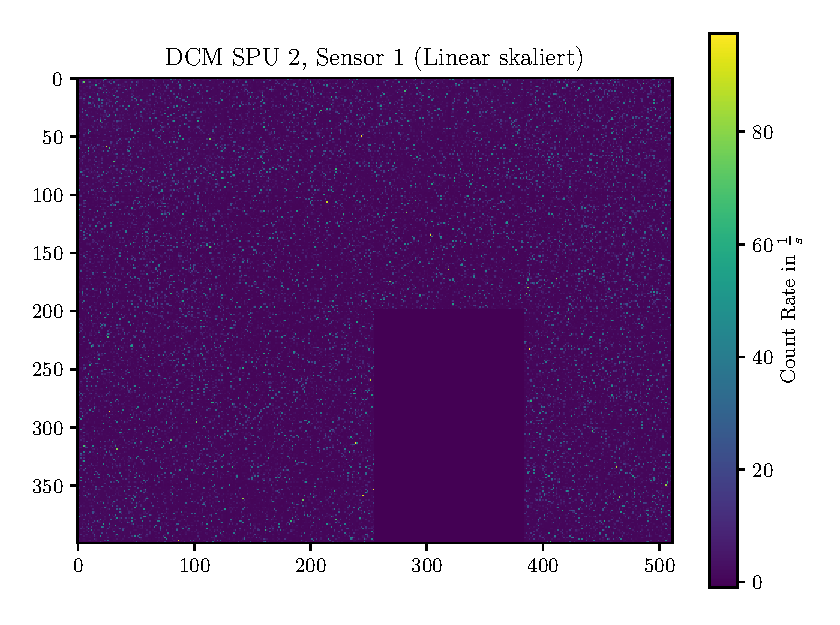
\includegraphics[width = \textwidth]{Plots/DCM/DCM_SPU2_Sensor1_lin.eps}
			\caption{DCM SPU 2, Sensor 1, Linear}
		\end{figure}

		\begin{figure}[H]
			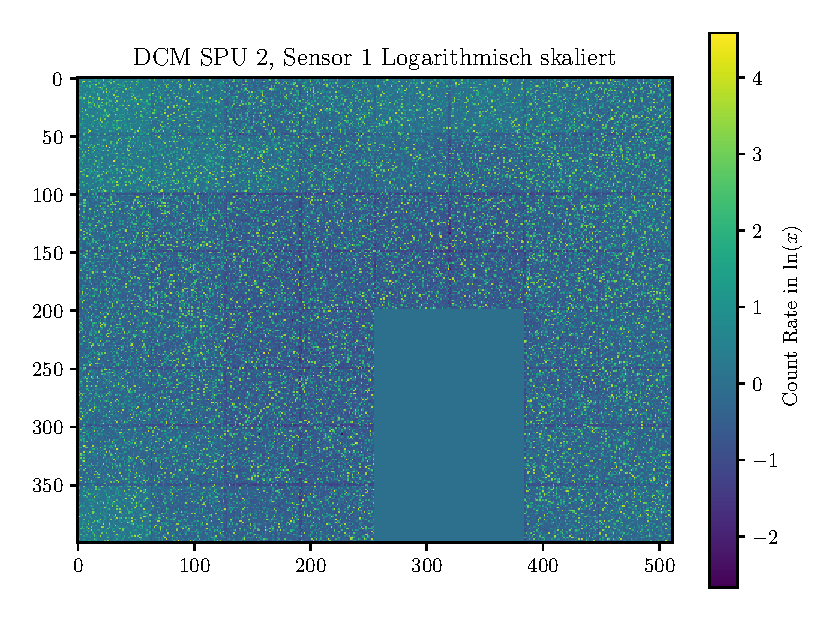
\includegraphics[width = \textwidth]{Plots/DCM/DCM_SPU2_Sensor1_log.eps}
			\caption{DCM SPU 2, Sensor 1, Logarithmisch}
		\end{figure}

		\begin{figure}[H]
			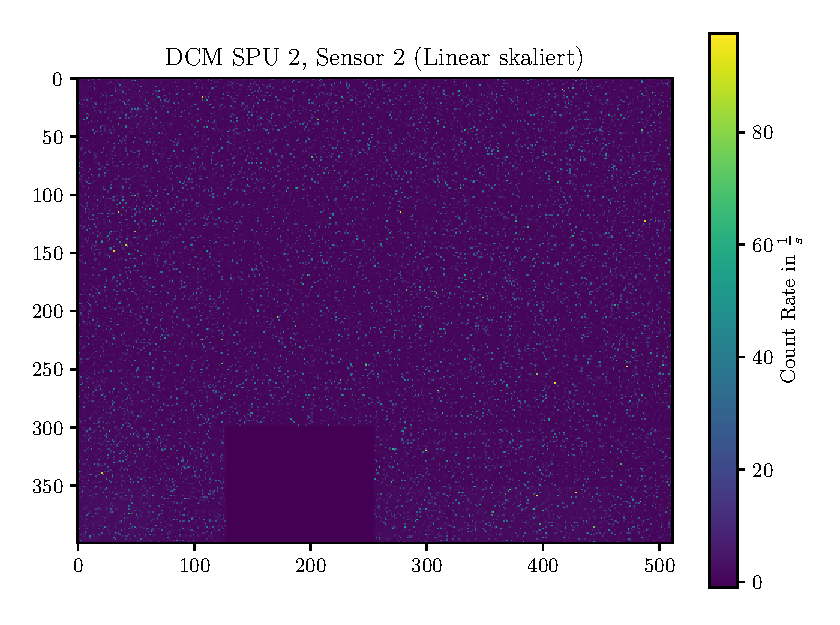
\includegraphics[width = \textwidth]{Plots/DCM/DCM_SPU2_Sensor2_lin.eps}
			\caption{DCM SPU 2, Sensor 2, Linear}
		\end{figure}

		\begin{figure}[H]
			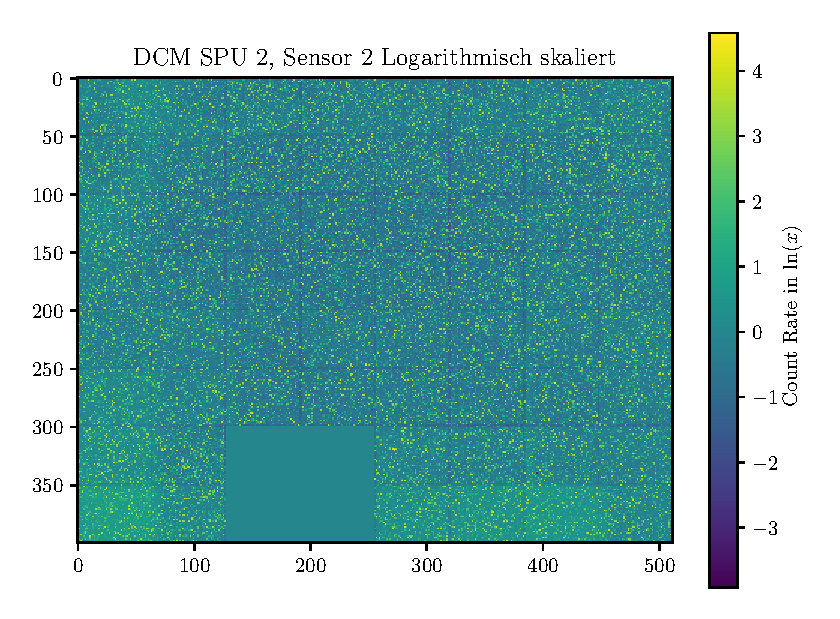
\includegraphics[width = \textwidth]{Plots/DCM/DCM_SPU2_Sensor2_log.eps}
			\caption{DCM SPU 2, Sensor 2, Logarithmisch}
		\end{figure}

\end{document}
